\documentclass[12pt]{galois-whitepaper}
\usepackage{listings}
\usepackage{float}
\usepackage{xspace}
\usepackage{color}
\usepackage{tikz}
\usepackage{url}
\usepackage{amsmath}
\usepackage{amsfonts}
\usepackage{amssymb}
\usepackage{amscd}
\usepackage{verbatim}
\usepackage{subcaption}
\usepackage{fancyvrb}
\let\verbatiminput=\verbatimtabinput
\VerbatimFootnotes
\DefineVerbatimEnvironment{code}{Verbatim}{}
\DefineVerbatimEnvironment{pseudoCode}{Verbatim}{}
%\hyphenation{Saw-Script}
%\newcommand{\sawScript}{{\sc SawScript}\xspace}

\usepackage[all,2cell]{xy}
\UseAllTwocells

\usepackage{textcomp}

\renewcommand{\textfraction}{0.05}
\renewcommand{\topfraction}{0.95}
\renewcommand{\bottomfraction}{0.95}
\renewcommand{\floatpagefraction}{0.35}
\setcounter{totalnumber}{5}
\definecolor{MyGray}{rgb}{0.9,0.9,0.9}
\makeatletter\newenvironment{graybox}{%
   \begin{lrbox}{\@tempboxa}\begin{minipage}{\columnwidth}}{\end{minipage}\end{lrbox}%
   \colorbox{MyGray}{\usebox{\@tempboxa}}
}\makeatother

\setlength{\parskip}{0.6em}
\setlength{\abovecaptionskip}{0.5em}

\lstset{
         basicstyle=\footnotesize\ttfamily, % Standardschrift
         %numbers=left,               % Ort der Zeilennummern
         numberstyle=\tiny,          % Stil der Zeilennummern
         %stepnumber=2,               % Abstand zwischen den Zeilennummern
         numbersep=5pt,              % Abstand der Nummern zum Text
         tabsize=2,                  % Groesse von Tabs
         extendedchars=true,         %
         breaklines=true,            % Zeilen werden Umgebrochen
         keywordstyle=\color{red},
                frame=lrtb,         % left, right, top, bottom frames.
 %        keywordstyle=[1]\textbf,    % Stil der Keywords
 %        keywordstyle=[2]\textbf,    %
 %        keywordstyle=[3]\textbf,    %
 %        keywordstyle=[4]\textbf,   \sqrt{\sqrt{}} %
         stringstyle=\color{white}\ttfamily, % Farbe der String
         showspaces=false,           % Leerzeichen anzeigen ?
         showtabs=false,             % Tabs anzeigen ?
         xleftmargin=10pt, % was 17
         xrightmargin=5pt,
         framexleftmargin=5pt, % was 17
         framexrightmargin=-1pt, % was 5pt
         framexbottommargin=4pt,
         %backgroundcolor=\color{lightgray},
         showstringspaces=false      % Leerzeichen in Strings anzeigen ?
}

\author{Eric Davis, Alec Theriault, and Ryan Wright}
\title{October ASKE Milestone Report for AMIDOL}
\date{10/31/2019}
\begin{document}
\maketitle

\vspace*{2cm}
\tableofcontents

\section{Introduction}

Recent work on AMIDOL has focused on preparation for the upcoming live
demo, and final code release, including adding features to update
AMIDOL's UI, prepare AMIDOL for internal evaluation as part of the
upcoming Milestone 12 report on system performance, and to extend the
theory underlying AMIDOL's representation of models, and layers of
abstraction.  The latter is particularly important for enriching
AMIDOL's ability to compose models.  We have released the
next version of AMIDOL at its github site
(\url{https://github.com/GaloisInc/AMIDOL/}) under the BSD 3-Clause
``New'' or ``Revised'' License.

\section{Model Representation and Abstraction}

AMIDOL is currently able to represent models in three separate
layers.  As formulations in the \textbf{Abstract Knowledge Layer}, and
displayed in the UI as a visual domain specific language; as process
algebras in the \textbf{Structured Knowledge Layer} - AMIDOL's
intermediate representation; and lastly as executable code synthesized
by AMIDOL's compiler stack, to generate results.

Models in AMIDOL are compositional, made up of many component parts,
but functioning as a whole unit that can be saved, loaded, edited,
shared, and executed, seemlessly transitioning across knowledge layers
of the metamodeling process.  We are currently extending these
capabilities and representations to better capture real-world
scientific goals and practices to allow user constructed models to
also serve as components of other models, in a process we refer to as
\textbf{model abstraction}.

For the sake of discussion, we refer to \emph{lower level} models and
\emph{higher level models} to distinguish relationships in compositional
hierarchies in AMIDOL with lower level models indicating a model with
a more detailed representation, and higher level models as models
which represent one or more low level models atomically.  Graphically,
this can be represented with a higher level model consisting of nodes
connected by edges, where some of the nodes in the higher level model
can be expanded to see the detailed implementation of lower level models.

This distinction between higher and lower-level model abstractions is
already prevalent throughout scientific communities. Chemistry models
are useful to chemists as such without having to always reduce the
chemical model to its fundamental quantum physics model.  Biochemical
models abstract the chemical formulas of proteins and other compounds,
and cellular models further abstract to the abstract machines of
cellular function.  While these abstractions help to simplify models
for consumption by domain experts, AMIDOL aims to unlock insights at
these lower levels, by allowing easy access to the underpinnings and
mechanics of abstractions.

We plan to explore how models at multiple levels of abstraction are
best represented formally and used for computation. Just as functions
in programming languages are composable, we expect model composition
to work through a system of well-defined inputs and outputs. The
inputs will have a structure defining the number and type of each
input argument. Outputs will also be similar structured. So a model
becomes composable and usable as a lower level model only when the
inputs and outputs are properly typed according to types representable
to the higher level model.  We reason about this typing using Applied
Category Theory, representing each lower level model as a morphism in
the higher level model \[X \nrightarrow Y.\]

  \begin{figure}
    \centering
    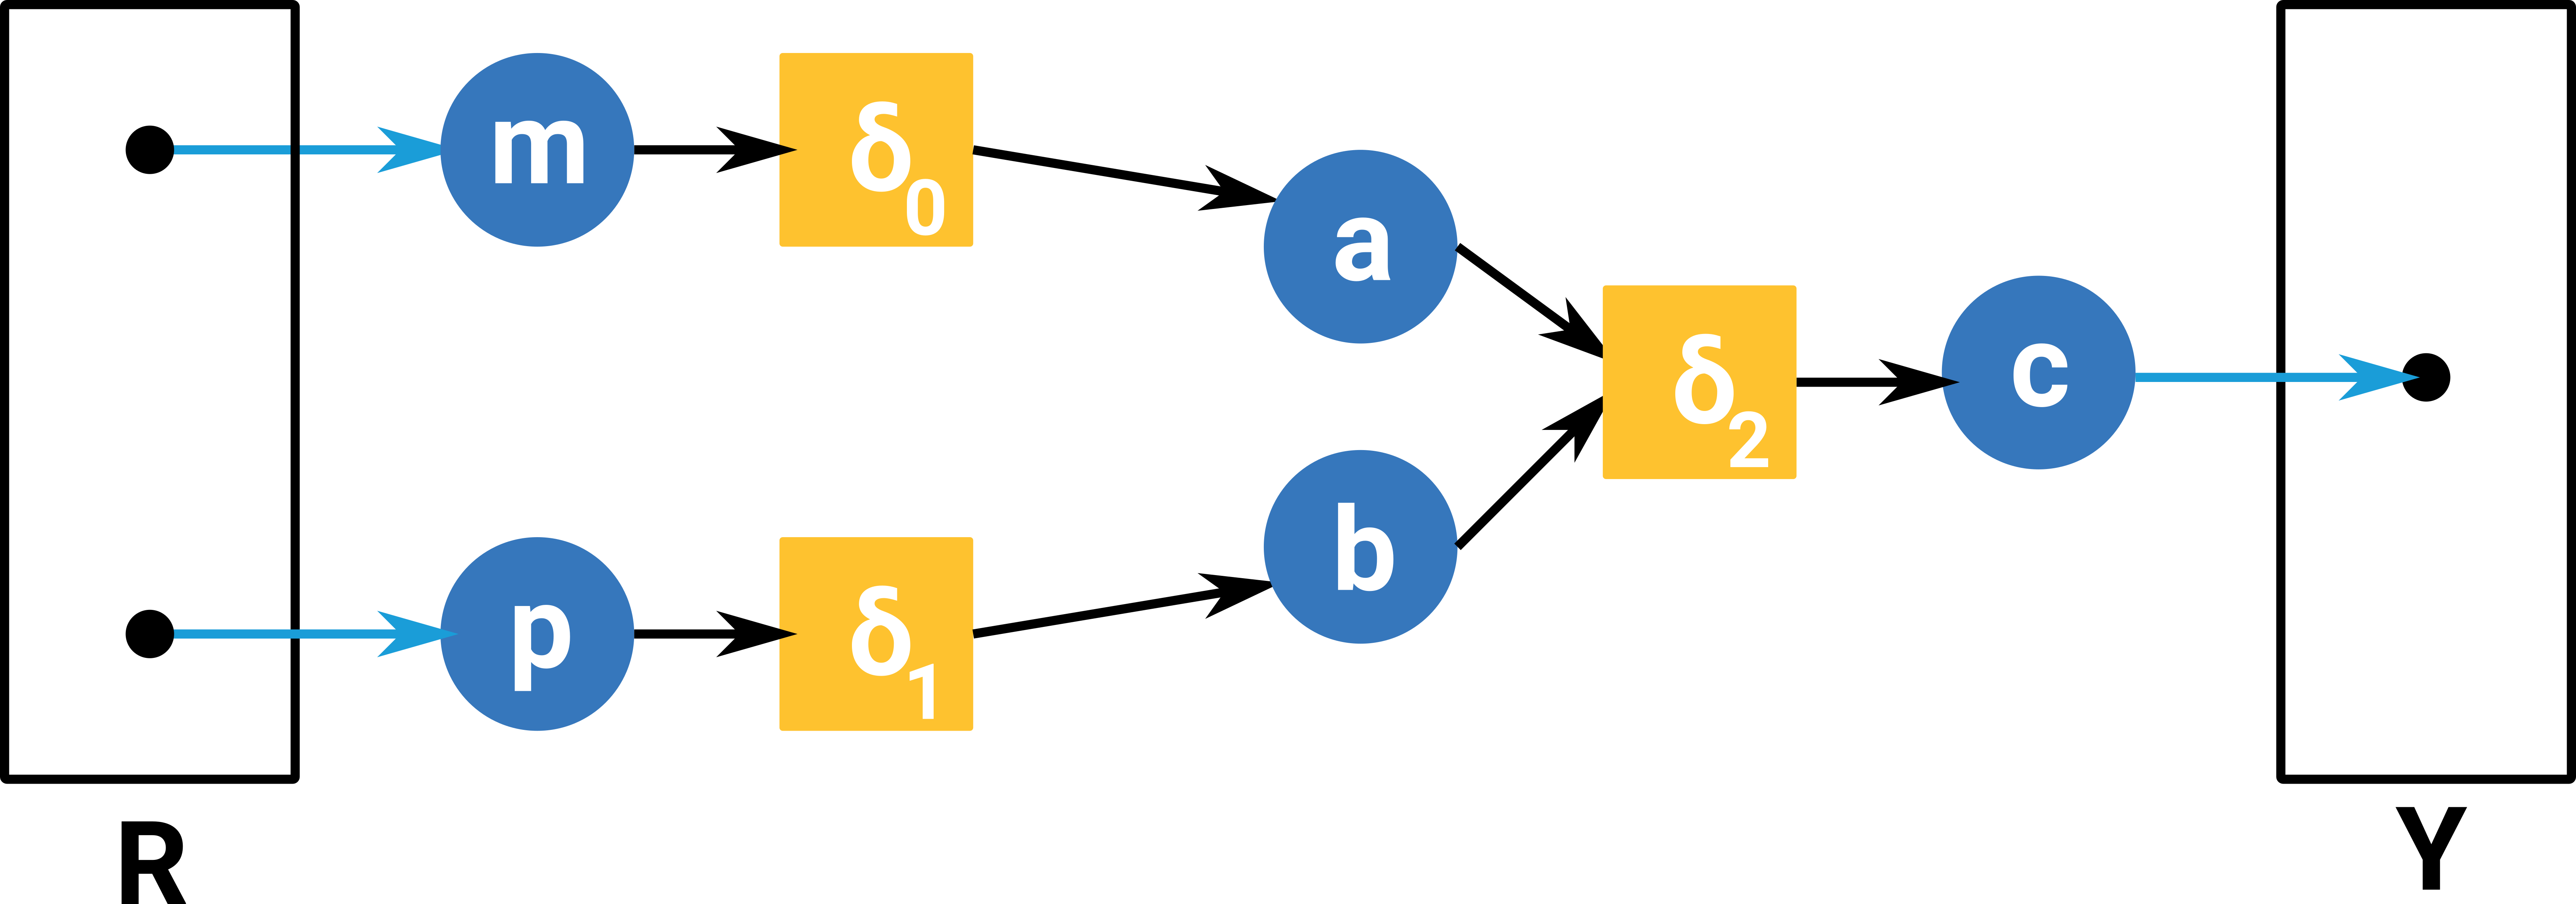
\includegraphics[width=\textwidth]{figs/series-2.png}
    \caption{AMIDOL Model Signatures}
    \label{Fig:Signature}
  \end{figure}

Figure \ref{Fig:Signature} illustrates how Applied Category Theory can
be used to learn the type of a lower level model.  Both the airty of
the inputs and outputs, and their domain typing (as inferred from
groundings in the formulation) inform this typing. As an example,
a lower level SIR model accepts as input a population of
susceptible people and produces as output three populations of
susceptible, infected, and recovered people. A higher level model
could include this lower level SIR model as a node in its graph if and
only if the higher level model

\begin{enumerate}
\item has types for susceptible, infected, and recovered persons,
\item can provide as input a susceptible population, and
\item accepts results from the lower level model node (as outgoing arrows)
  for at least one of the susceptible, infected, and recovered person
  populations.
\end{enumerate}

Depending on the lower level model, there may also be
additional constraints placed on the values of the types in
question. We plan to add support for these constraints in AMIDOL, and
to allow them to be saved as part of the model formulation to test
domain assumptions about generated models, and further help scientists
to both explore assumptions about their problem space; and to help
automatically enforce assumed constraints to reduce the chance of
error in model design and execution.

AMIDOL will allow higher level models to import lower level models as
part of its palette.  Higher level models, as models themselves, can
also be imported by additional, higher level, models.  This allows
recursive model composition and design to a high degree, and the
design of hierarchical palettes for model formulation leveraging prior
work, and found models from the literature.

\subsection{Model Comparison}

AMIDOL is implementing mechanisms to execute model comparisons using a
graph-based results database.  While individual scientific models may
be useful for describing complex systems, comparing two models with
different assumptions presents several challenges.
Quantum Theory and Relativity are probably the most famous examples of
this fact. In a fully realized AMIDOL system, two incommensurable
models could be analyzed in several productive ways. The AMIDOL system
could eventually deploy abilities for trace generation, analyzing the
way constraints and assumptions propagate throughout a model, exposing
invalid constraints when found, and providing counter examples which
help diagnose their interaction with the sub-components of a model.
This would allow domain scientists to better understand when and where
certain constraints apply to a model, under what inputs they do not
apply, and what portions of lower level models might violate
constraints, aiding the scientist in debugging and checking deeply
nested compositions of models.  While powerful, and novel for model
construction there exists a significant body of prior work to motivate
this capability, and suggest its feasibility.  Similar constraint
solving is currently accomplished by type checkers in programming
languages type systems.

\subsection{Learning Approximations}

Due to the potential computational intractability of systems composed
of highly nested model abstractions, we are investigating the ability
of AMIDOL to learn approximations of abstracted components.  As an
example, consider a model of neural structures in the brain.  While
the behavior of these structures is defined by the atomic reactions
occuring at each synapse, simulating a large collection of neural
tissue at the atomic level would take an unacceptably long period of
time due to the stiffness of the resulting model.  To provide value
for scientific research, modeling efforts need to deploy methods that
accommodate the stiffness of models.

Mathematically, a stiff model represents a system for which certain
numerical methods for solving the equation are numerically unstable,
often due to measure-relevant events in the system having wildly
different time-scales of occurance forcing the solution method to
utilize an extremely small step size.  Systems composed of many layers
of lower-level systems have an inherently higher risk of stiffness in
the final model, requiring intelligent methods for optimizing their solution.
We expect we will need to create methods for approximating lower level
model evaluations in these cases to improve solution techniques by
constructing a \emph{similar} model which is as indistinguishable as
possible in terms of black-box behavior, to the original fully defined syste,.
While this problem itself is its own area of independent research, we
hope to use model comparison to collect data from previous model runs
in the AMIDOL results database to improve empirical methods for
learning approximations.

\subsection{Integrating Data}

To support these new capabilities, we are extending AMIDOL by building
a data storage layer which is able to store, recall, organize, and
manage the results of previous model execution; and to store these
results as first class objects along with real-world measurements and data.
Because of the flexibility of a schema-less structure and expressive
query abilities, we’ve chosen a graph database as the fundamental
storage tool for AMIDOL, and we are working to define an algebra over
a field of these objects to allow their composition, comparison, and
manipulation by domain scientists in ways that are provably correct by construction.

\section{Progress Towards Live Demo and Final Code Release}

  \begin{figure}
    \centering
    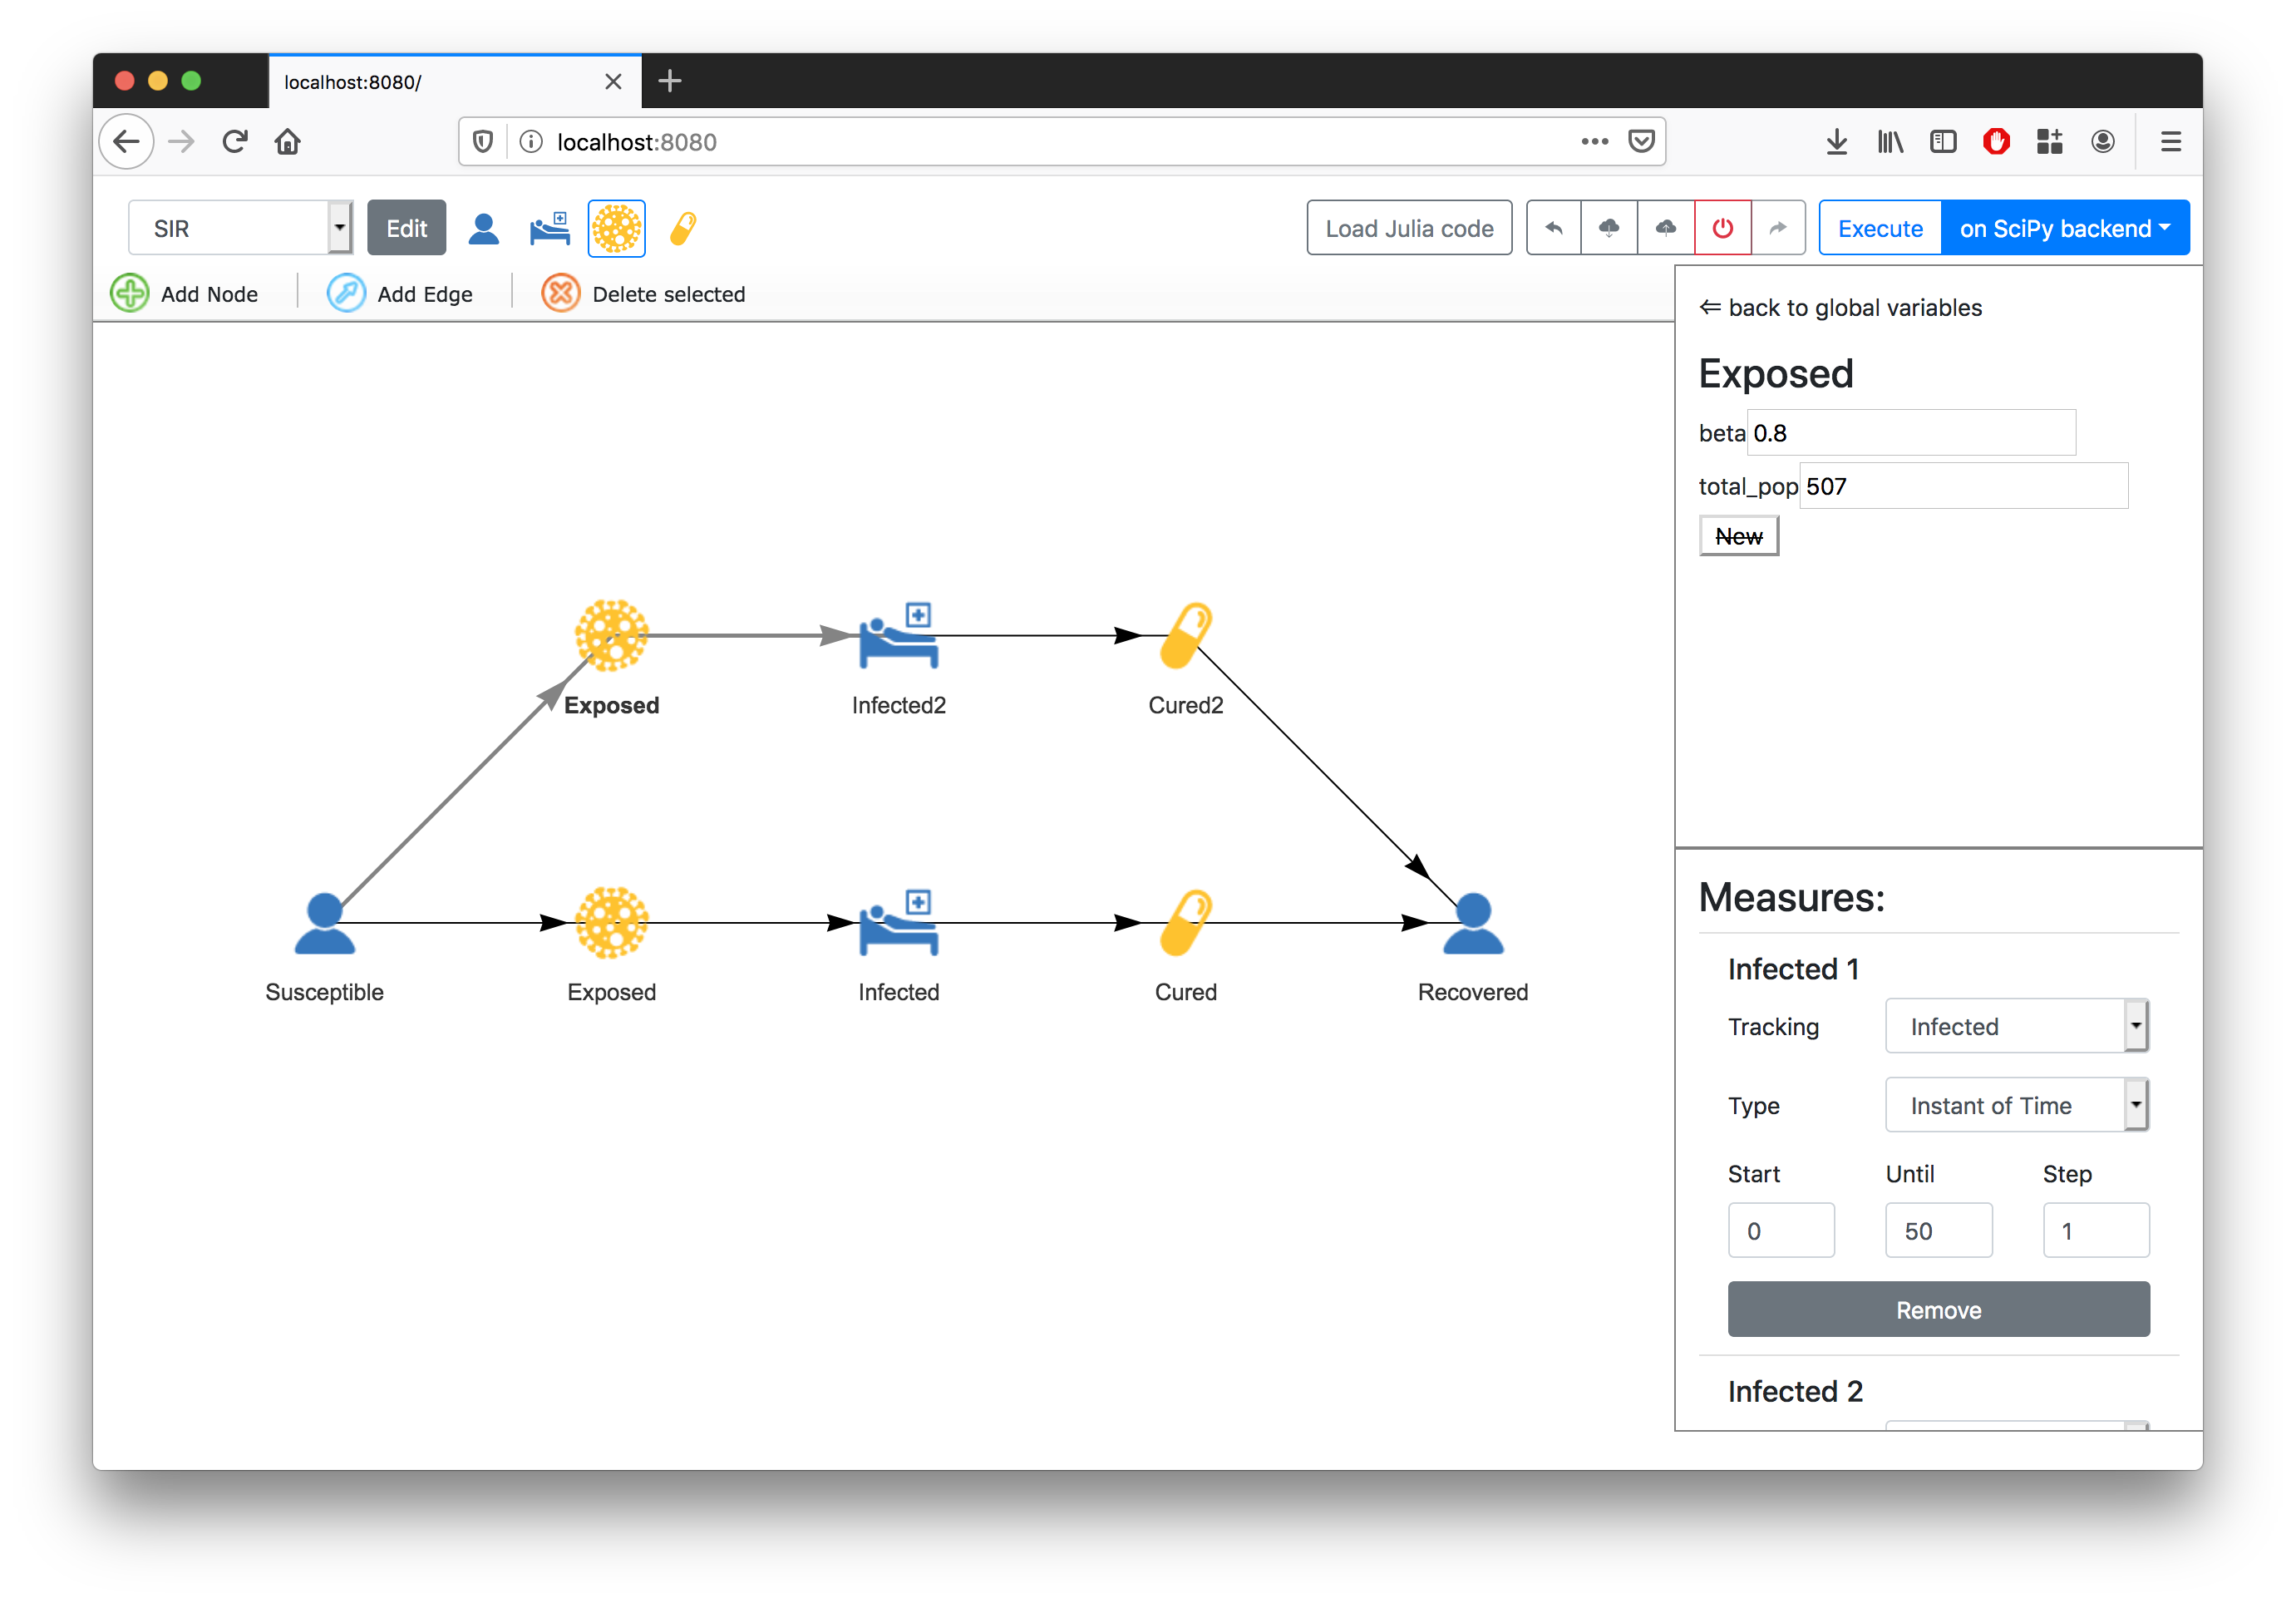
\includegraphics[width=\textwidth]{figs/mainscreen.png}
    \caption{New AMIDOL Main Screen}
    \label{Fig:MainScreen}
  \end{figure}

As the AMIDOL project has grown, the UI component has become
increasingly complex. When we first started, the web component
consisted of a single webpage, with all CSS and JavaScript inline, and
using a handful of standard libraries (jQuery, Underscore.js,
vis.js). This approach has not scaled well: adding a new feature takes
much longer than it used to and the risk of something being
accidentally broken is much higher. To address this problem, we’ve
been incrementally re-writing our UI to take advantage of modern
web-development technologies.

\begin{figure}
    \centering
    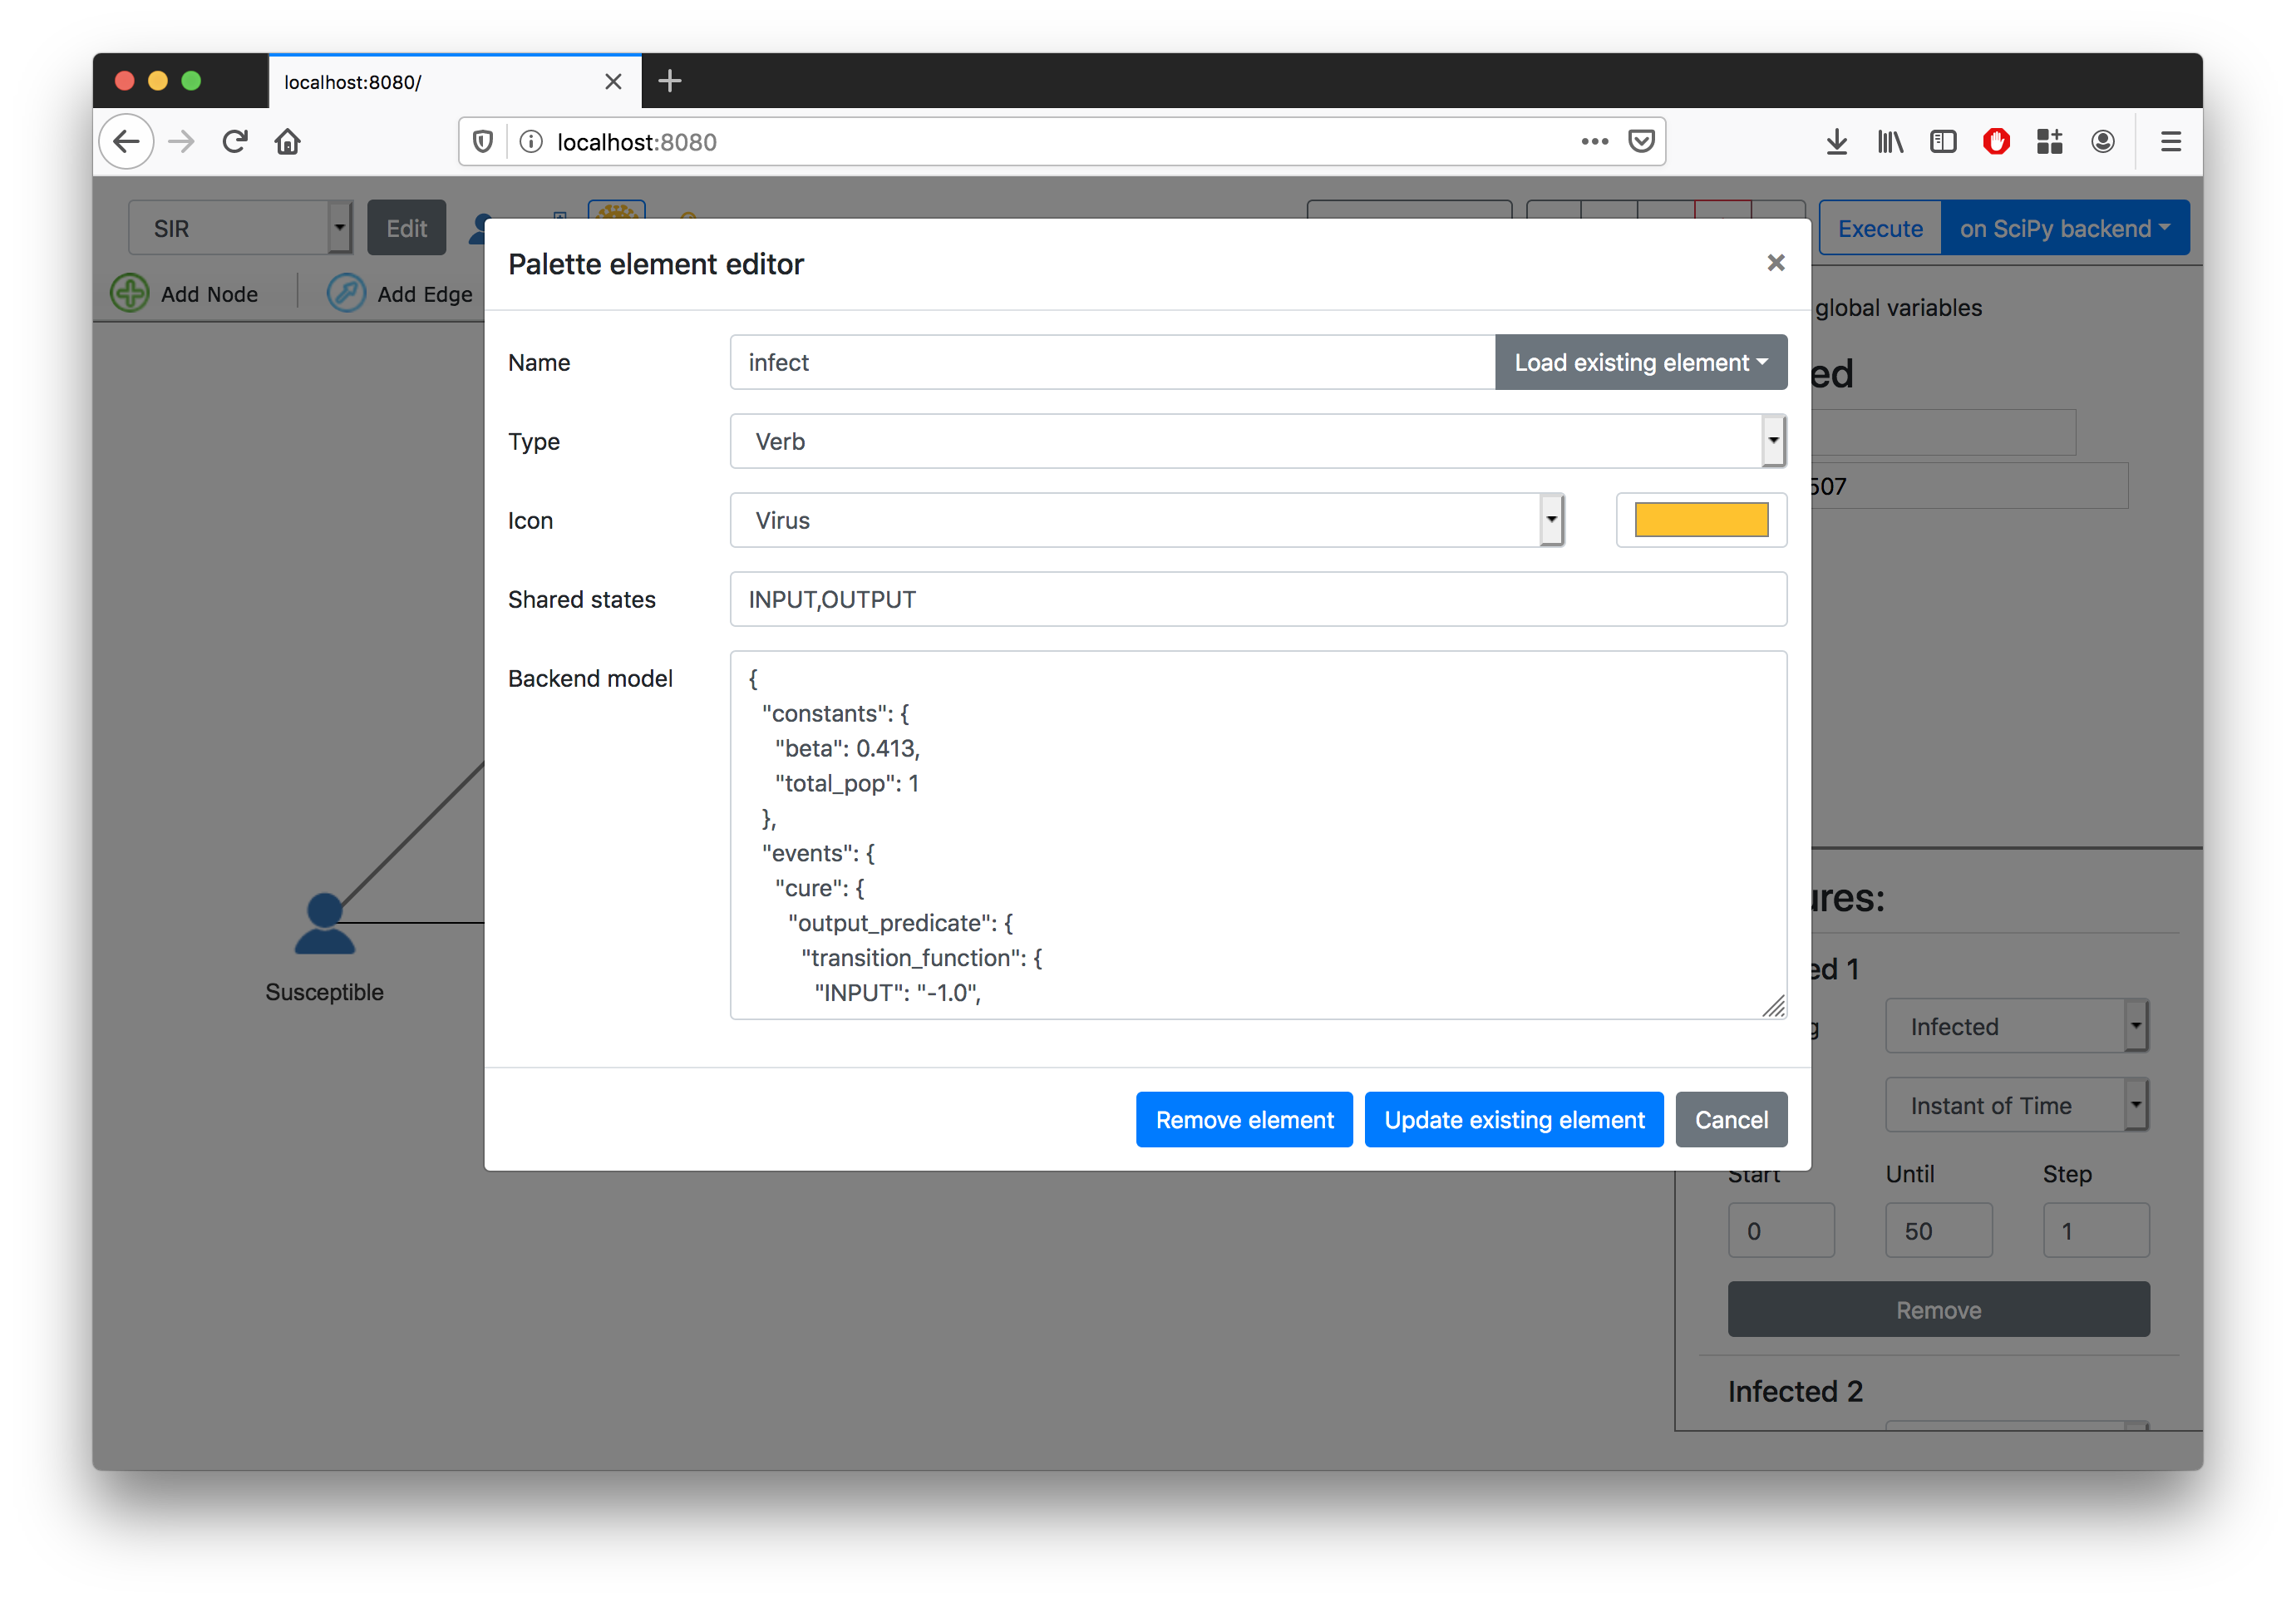
\includegraphics[width=\textwidth]{figs/palette.png}
    \caption{New AMIDOL Palette Editors}
    \label{Fig:PaletteScreen}
  \end{figure}

The first of these technologies is React, which is a framework for
building reusable UI components in a more declarative
fashion. Programmers can
describe how something is to be rendered, and React handles figuring
out when to re-render and how to stitch rendered outputs
together. Since React is widely used, we’ve also been able to take
advantage of other existing libraries which provide polished basic UI
elements with simple interfaces (things like pop-up modals, button
strips, list views, loading icons).

AMIDOL has also started using Typescript, which is a superset of JavaScript
that adds type annotations. This mostly helps build confidence that
some code change we make isn’t silently breaking something
else. Development is also much faster since we can take advantage of
type-driven IDE features (eg. type-aware completions).

  \begin{figure}
    \centering
    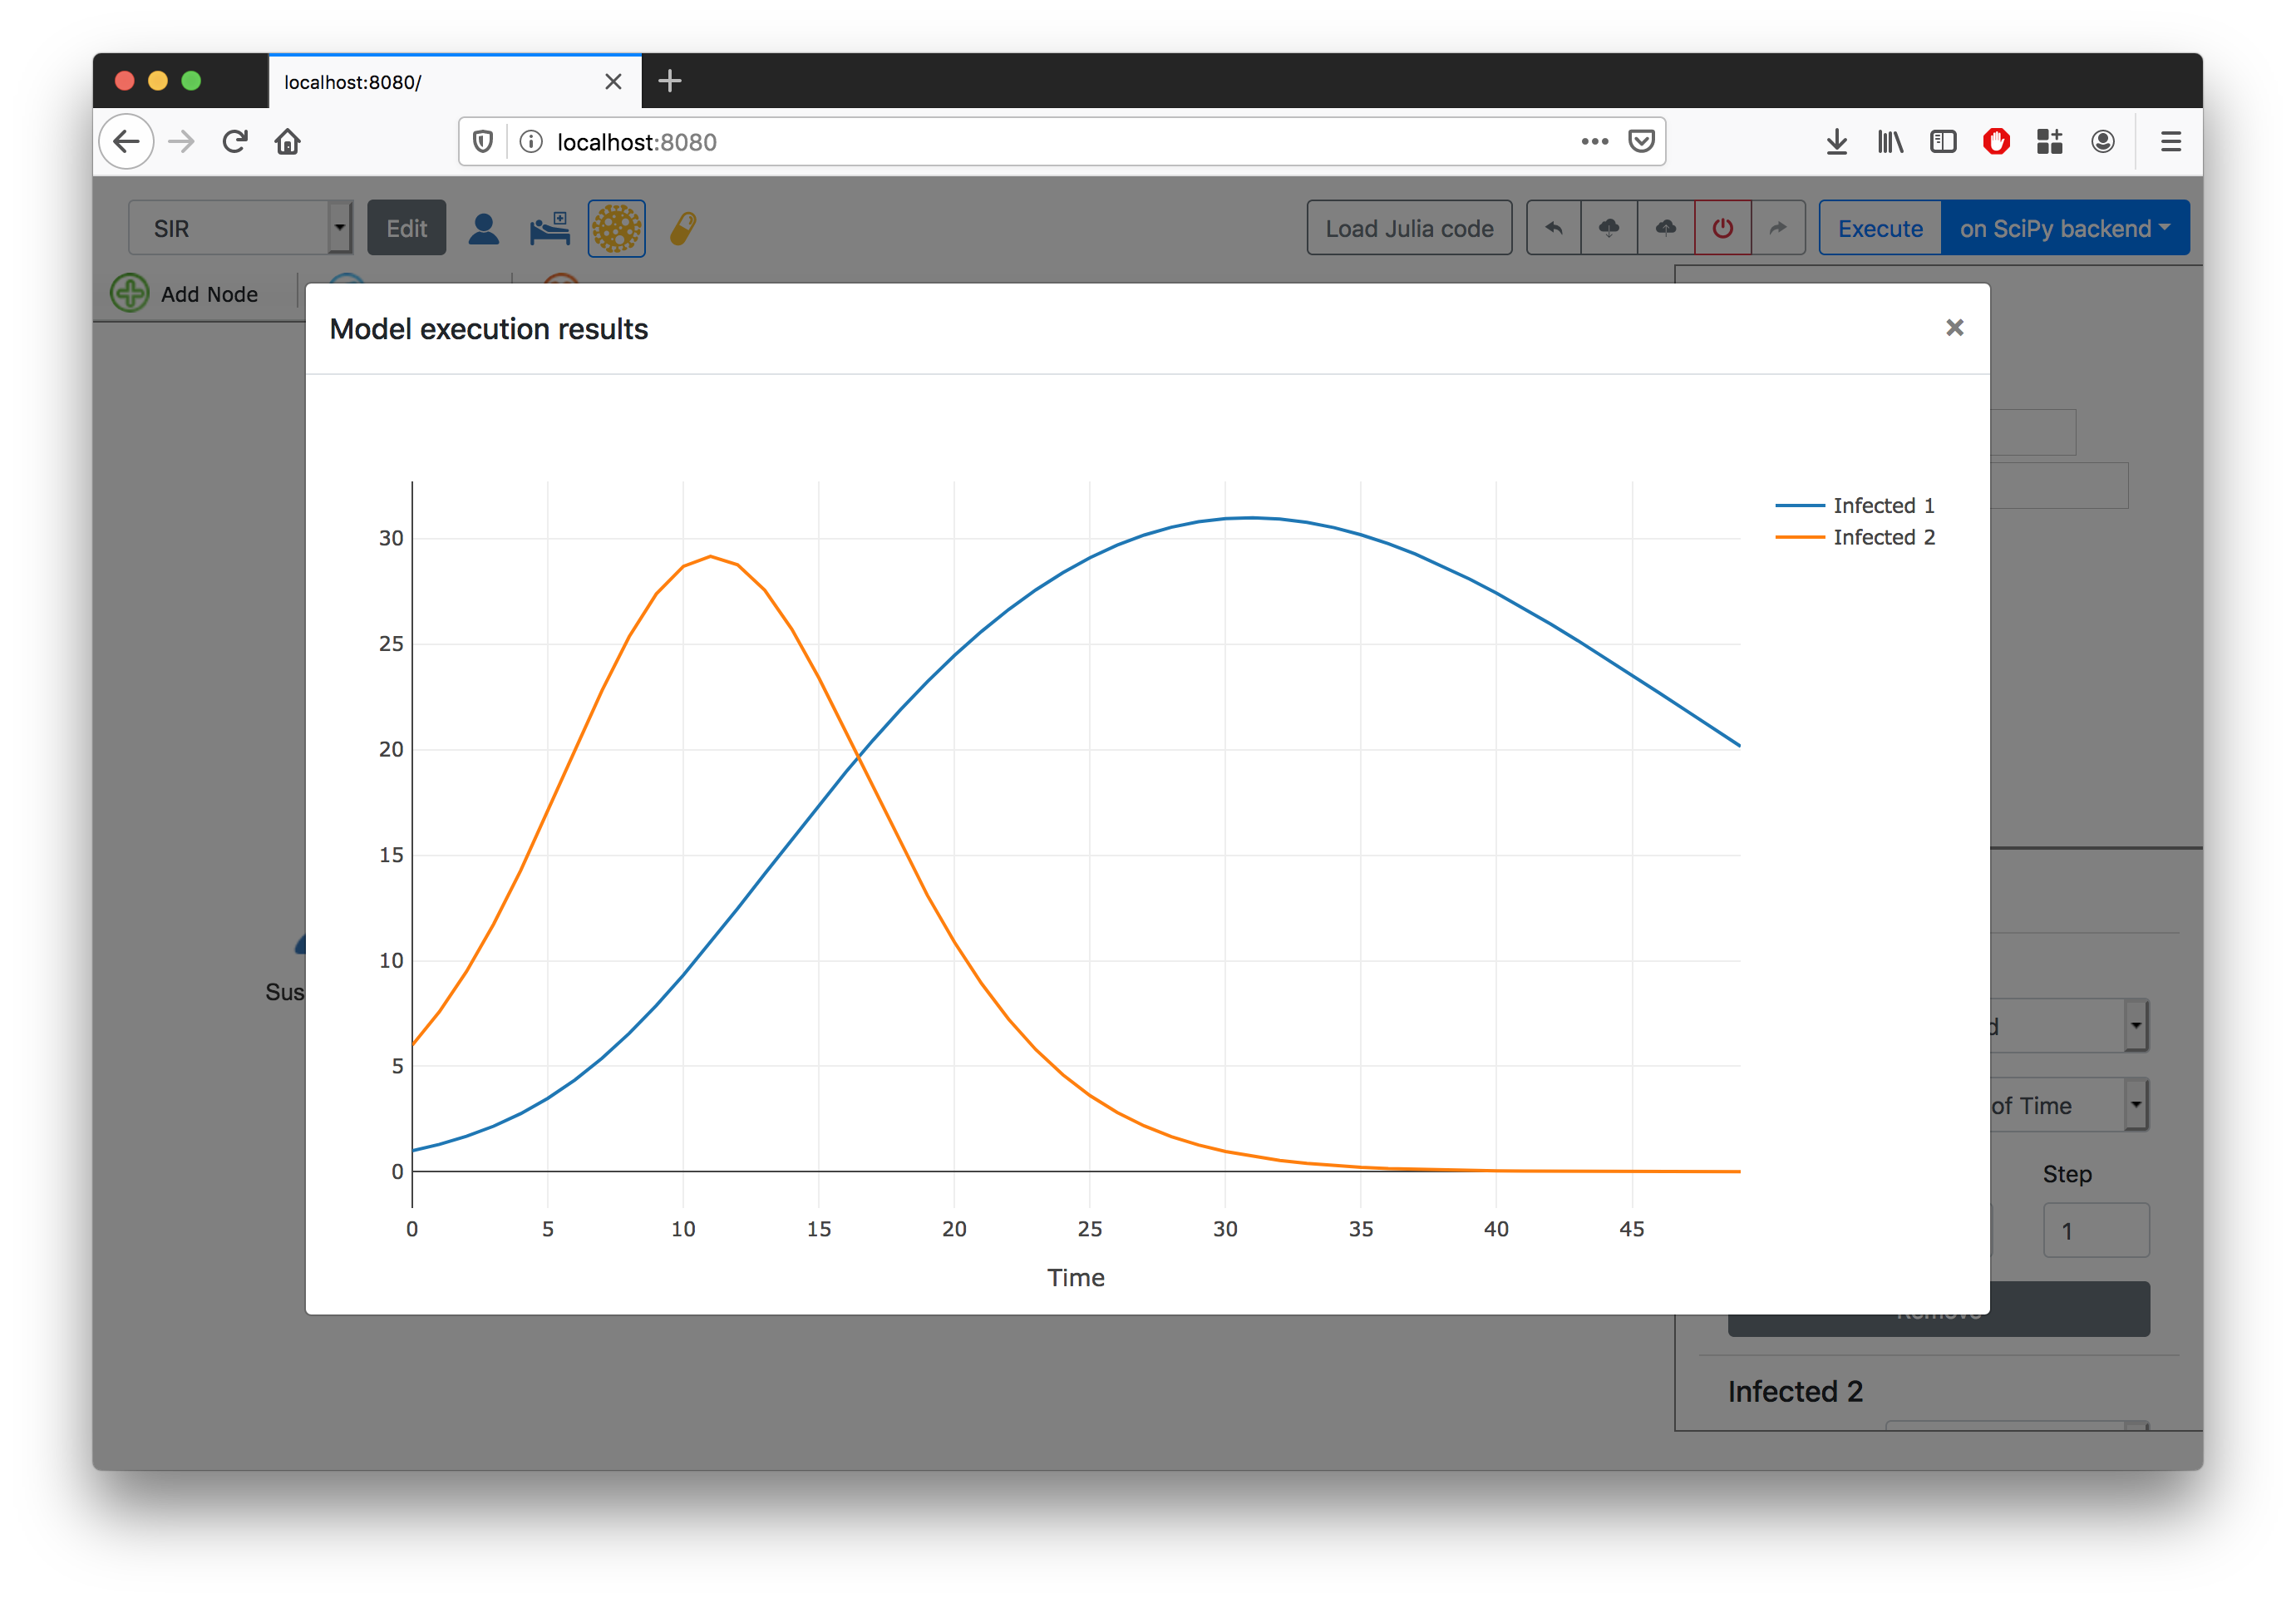
\includegraphics[width=\textwidth]{figs/results.png}
    \caption{New AMIDOL Results Screen}
    \label{Fig:ResultsScreen}
  \end{figure}

The final tool we’ve started using is Webpack. Since we’d like our UI
to work on a wide array of browsers, it is necessary to make sure that
the JavaScript we write doesn’t rely on features that are too new or
not cross-browser compatible. Webpack is the glue that holds the new
AMIDOL UI together: it takes our many Typescript code files and compiles
and minifies them into one portable JavaScript file, making the
eventual task of distributing AMIDOL to a wider audience of users easier.

As of today, almost all of our UI has been re-written in this new
stack. In the process, we’ve managed to fix a slew of small
issues. The new UI feels more polished and has a consistent
theme. Most importantly, we feel confident that we can quickly extend
it in new ways. Concrete next goals in this direction include
supporting other visual languages as well as providing more of a
modeling “workbench” experience.
  
\end{document}
